\documentclass[11pt]{article}
\usepackage[margin=1in]{geometry}
\usepackage[T1]{fontenc}
\usepackage[utf8]{inputenc}
\usepackage{newtxtext,newtxmath}
\usepackage{graphicx,booktabs,array,multirow,amsmath,siunitx,xcolor}
\usepackage[authoryear,round]{natbib}
\usepackage[hidelinks]{hyperref}
\usepackage{microtype}
\usepackage{lineno}
\usepackage{setspace}
\graphicspath{{images/}}
\setlength{\emergencystretch}{3em}
\linenumbers

\title{Evaluations of News Source Strategies to Disseminate Fake News in X}
\ifdefined\ANONYMOUS
  \author{Anonymous authors}
\else
  \author{Paul Leger\textsuperscript{a}\thanks{Corresponding author: \href{mailto:pleger@ucn.cl}{pleger@ucn.cl}; ORCID: \href{https://orcid.org/0000-0003-0969-5139}{0000-0003-0969-5139}} \and
  Agustín Olivares\textsuperscript{b} \and Oswaldo Teran\textsuperscript{c,d} \and
  Manuela Lopez\textsuperscript{e} \and Francis Espinoza\textsuperscript{b} \and
  Carolina Rodríguez\textsuperscript{f}\\[0.8em]
  \small \textsuperscript{a}Escuela de Ingeniería, Universidad Católica del Norte, Chile\\
  \small \textsuperscript{b}Universidad Católica del Norte, Chile\\
  \small \textsuperscript{c}Escuela de Ciencias Empresariales, Universidad Católica del Norte, Chile\\
  \small \textsuperscript{d}Centro de Simulación y Modelos (CESIMO), Universidad de Los Andes, Venezuela\\
  \small \textsuperscript{e}University of Murcia, Spain\\
  \small \textsuperscript{f}Universidad de La Serena, Chile}
\fi
\date{}

\begin{document}
\maketitle
\begin{abstract}
Malicious news sources can change their presentation without changing the probability that their publications are false. This study evaluates such strategies in X through a survey-informed agent-based model. Five hundred heterogeneous users repeatedly select and repost publications from four source types according to accumulated evaluations, visibility, social recommendations, and memory. Malicious sources imitate engagement, proximity, information-quality, and credibility attributes of traditional media. We conduct 2,010 seeded runs across four experiments concerning strategy type, campaign timing and duration, reach restrictions, and behavioural sensitivity. Strategies increased the malicious source's audience, especially when all attribute groups were imitated, but generally produced small changes in the overall share of false reposts under truth-sensitive recommendations. Reach restrictions reduced malicious-source participation and eliminated strategy effects at zero direct reach. Truth-sensitive recommendations attenuated the additional false-repost effect observed when recommendations were disabled. Sensitivity analysis showed that audience-capture conclusions were robust, whereas false-repost effects depended on memory persistence. The findings distinguish source success from societal misinformation exposure and suggest evaluating reach governance and recommendation mechanisms jointly. The model is a policy-oriented computational laboratory rather than a predictive representation of X.
\end{abstract}

\noindent\textbf{Keywords:} agent-based modelling; fake news; misinformation; news sources; social media; scenario analysis

\section{Introduction}

Fake news can impose costs well beyond an isolated inaccurate belief. In democratic settings, disinformation can distort public debate, intensify polarisation, and erode trust in elections, institutions, and journalism; the OECD therefore treats information integrity as an enabling condition for democratic participation and accountable government \citep{oecd2024}. Public-health decisions provide a second concrete example. In a randomised experiment in the United Kingdom and the United States, exposure to COVID-19 vaccine misinformation reduced the share of respondents who said they would definitely accept vaccination by 6.2 and 6.4 percentage points, respectively \citep{loomba2021}. These examples do not imply that every false publication changes behaviour or determines an election. They show why the reach and repetition of deceptive content can create societal consequences that justify careful, rights-aware intervention.

Online social networks allow news sources to reach large audiences with low publication and redistribution costs. The same infrastructure supports legitimate journalism, uncertain information, deliberately deceptive content, and mixtures of these forms. False news has been shown to diffuse farther and faster than true news in large Twitter cascades \citep{vosoughi2018}, while exposure and sharing are concentrated among subsets of users \citep{grinberg2019,guess2019}. These findings motivate interventions, but they do not by themselves reveal how a malicious source may adapt its observable presentation when platforms or users become more selective.

This paper focuses on strategies controlled by a news source that repeatedly disseminates false publications. Such a source may imitate attributes associated with established media: emotional engagement, political or social proximity, apparent information quality, or source credibility. We distinguish these perceived attributes from the objective probability that a publication is false. This separation is essential. A camouflage strategy can make a source more attractive without making its output more accurate. We use \textit{false news} for factually false news-like publications, \textit{misinformation} without assuming intent, and \textit{disinformation} only when deliberate deception is established. Because the model specifies behaviour rather than an internal intention state, ``malicious source'' is shorthand for the experimental source and not an empirical diagnosis of motive.

Observed social-media data are indispensable but make controlled counterfactuals difficult. Agent-based modelling (ABM) complements observation by representing users with heterogeneous states and network positions, repeated decisions and feedback, and by changing one policy or strategy while holding the remaining design constant \citep{macal2010,grimm2020}. Our model therefore serves as a computational laboratory for source strategies and mitigation policies; it is not intended to forecast X at the individual-user level.

We address four research questions:

\begin{description}
\item[RQ1.] How do source-imitation strategies affect malicious-source reach and fake-news dissemination? Platforms and users observe many source characteristics, but it is unclear which groups of characteristics are most exploitable or whether a source gaining audience necessarily increases network-wide false-news exposure. RQ1 contributes a controlled ranking of individual and combined imitation strategies while holding objective fake-news probability fixed.
\item[RQ2.] How do campaign timing and duration affect efficacy and persistence? Deceptive presentation may be adopted early, late, or temporarily, while detection and intervention occur after different delays. A full-run average confounds start time with exposure duration, so RQ2 contributes matched treatment and post-removal windows that distinguish opportunity during a campaign from persistence after it ends.
\item[RQ3.] How effectively does limiting experimental-source reach mitigate dissemination, and how do recommendation policies modify this relationship? Reach and recommendation are platform-controllable mechanisms, but interpersonal diffusion could complement or bypass direct visibility restrictions. An immediate and perfectly truth-aware mechanism is an informative boundary, not a realistic platform description. RQ3 therefore contributes a joint assessment of graded reach limits, discovery-only recommendation, asymmetric flagging, delayed and imperfect labels, and recommendation magnitude.
\item[RQ4.] Are strategy conclusions robust to parameter and structural uncertainty? Memory persistence and contact counts are uncertain behavioural assumptions rather than direct policy levers, and conclusions may also depend on source behaviour, choice scaling, user activity and network construction. RQ4 contributes local, global and structural sensitivity analyses that distinguish stable conclusions from effects requiring stronger behavioural qualifications.
\end{description}

The contribution is threefold. First, we provide a modular ABM in which named source strategies selectively copy observable attributes while publication veracity remains unchanged. Second, we use common random-number seeds in a staged computational experiment to compare strategy, timing, reach and recommendation policies and to screen parameter and structural uncertainty. Third, we distinguish four outcomes that policy discussions can otherwise conflate: false reposts per agent-period, false reposts among actual decisions, experimental-source share among decisions, and participation.

The remainder of the paper is organised as follows. Section~2 reviews fake-news dissemination, ABM, and related simulation applications. Section~3 describes the model and experimental design using the ODD protocol. Section~4 reports the four research-question analyses. Section~5 documents software verification and conceptual and behavioural validation. Section~6 develops societal and policy implications while delimiting the claims supported by the experiments. Section~7 concludes and identifies the next validation steps.

\section{Background: fake news and simulation models for analysing its dissemination}

This section establishes the conceptual and methodological foundations of the study. It first explains why fake-news dissemination is mediated by source identity and social interaction, then introduces ABM and the ODD reporting protocol, and finally positions the proposed model relative to existing misinformation simulations.

\subsection{Fake news and source-mediated dissemination}

Fake news is not merely erroneous information; it is fabricated content presented in a news-like form and connected to incentives, attention, and institutional trust \citep{lazer2018,allcott2017}. Social platforms alter the route by which people encounter this content. Users select from sources, observe peers, and react to signals such as credibility, emotional tone, familiarity, and proximity. Homophilous communities can reinforce selective exposure \citep{delvicario2016}, and social influence can change evaluations independently of intrinsic quality \citep{muchnik2013}.

Source identity matters because users often lack the time or information needed to verify each claim. Aggregated judgments of source quality can support misinformation interventions \citep{pennycook2019}, whereas low-credibility content may receive coordinated amplification from automated accounts \citep{shao2018}. These mechanisms make source-level policies---visibility limits, recommendation rules, labels, and sanctions---plausible levers. They also create adaptation incentives: a malicious source may modify visible attributes to resemble a trusted source.

\subsection{Agent-based models as simulation models}

ABMs describe system outcomes as the emergent result of local decisions and interactions. They are useful when agents differ, remember past events, learn from contacts, and respond to interventions over time. In social-network research, \ifdefined\ANONYMOUS related prior applications are withheld for blinded review.\else ABMs have evaluated word-of-mouth (WOM) campaigns and participant selection \citep{leger2016,plaza2019}, message repetition on Twitter \citep{lopez2023}, and extensible architectures for social-network simulation \citep{leger2026}.\fi{} These applications illustrate how an executable mechanism can connect individual exposure and choice to population-level diffusion while retaining a controlled experimental design.

A credible ABM must make its entities, processes, scheduling, stochasticity, inputs, and outputs explicit. We follow the ODD protocol \citep{grimm2020}, which organises a model description into Overview, Design concepts, and Details. Figure~\ref{fig:odd} summarises how those components move from the scientific purpose and system boundary to behavioural assumptions and executable submodels. ODD supports inspection and replication, but does not itself establish that a model is valid for every use.

\begin{figure}[ht]
\centering
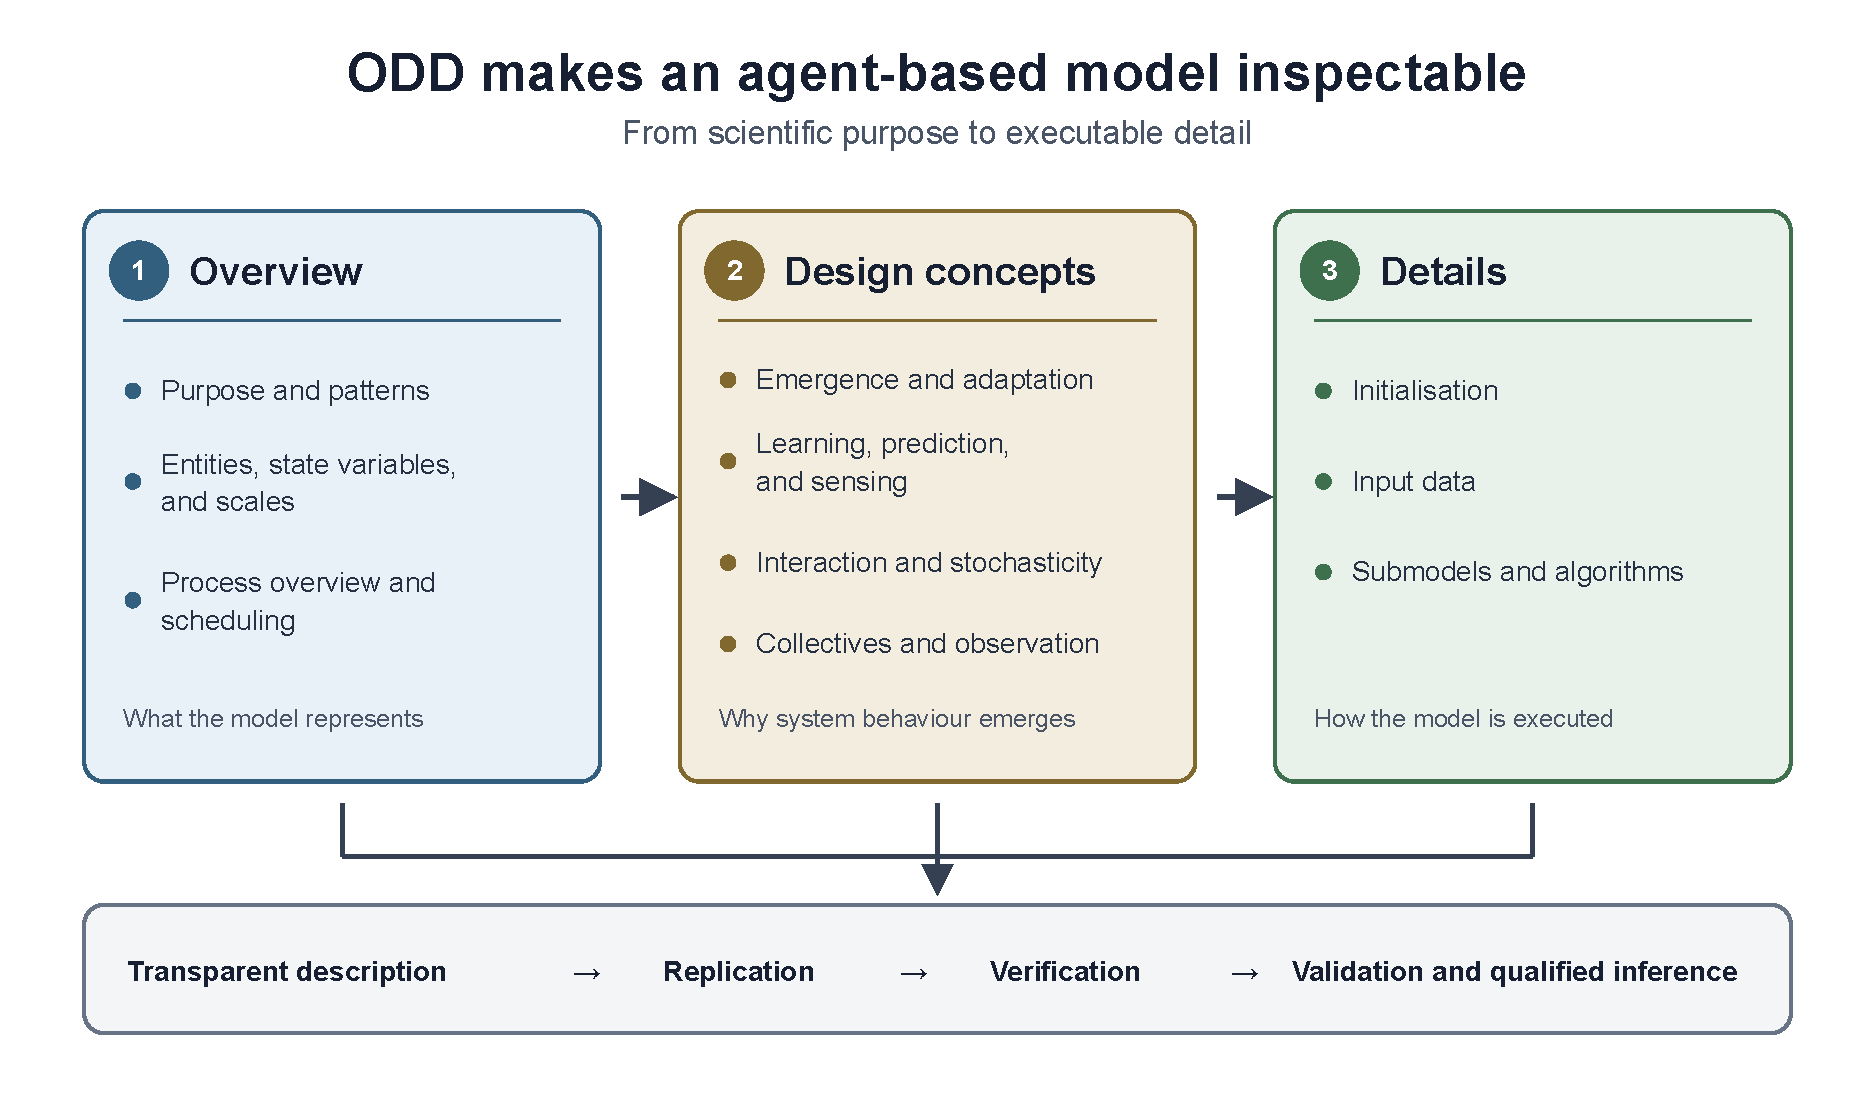
\includegraphics[width=.98\linewidth]{odd-protocol-abm.pdf}
\caption{Original synthesis of the ODD protocol for documenting an agent-based model. The three descriptive components support replication, software verification, and qualified validation.}
\label{fig:odd}
\end{figure}

Simulation evidence has a different status from observational or experimental evidence about people. A simulation supports conditional statements: given the encoded mechanisms and parameter ranges, a strategy produces a measured change. Verification asks whether the software implements that specification; validation asks whether the representation is sufficiently credible for its intended purpose. Neither process turns an exploratory model into a direct prediction of platform behaviour.

\subsection{Simulation models of misinformation}

Misinformation models range from epidemic analogies to network, opinion-dynamics, and cognitively richer agent systems. Table~\ref{tab:related-models} compares representative models by their behavioural focus, empirical input, intervention and validation. Competing-rumour models represent misinformation and fact-checking as diffusion processes \citep{sulis2020}; game-theoretic models examine deception and cooperation \citep{hills2018}; curation models connect belief, recommendation objectives and empirically observed Twitter data \citep{gausen2022}; and bot models study how network position changes indirect influence \citep{keijzer2021}. Recent work also reconstructs language and network histories through digital cloning \citep{puri2024}, examines moderation across platforms \citep{murdock2024}, and evaluates governance in decentralised systems \citep{malgonde2025}.

\begin{table*}[ht]
\centering
\caption{Positioning relative to representative misinformation simulation models. ``Empirical'' identifies inputs or validation data reported by each study; it does not imply predictive validity.}
\label{tab:related-models}
\small
\begin{tabular}{p{2.5cm}p{2.8cm}p{2.6cm}p{2.5cm}p{3.4cm}}
\toprule
Study & Main mechanism & Network/input & Intervention & Distinctive analytical focus \\
\midrule
\citet{sulis2020} & Competing misinformation and debunking states & Configurable synthetic networks & Fact-checking probability & Diffusion and forgetting \\
\citet{hills2018} & Evolutionary deception and cooperation & Random interactions; empirical pattern comparison & Behavioural costs & Deception types and cooperation \\
\citet{gausen2022} & Beliefs and newsfeed curation & Parameterisation and case comparisons using Twitter data & Curation objectives & Algorithmic misinformation--polarisation trade-off \\
\citet{keijzer2021} & Cultural influence by bots and humans & Synthetic network structures & Bot activity and connectivity & Direct versus indirect bot influence \\
\citet{puri2024} & Language-sensitive digital clones & Observed network and message histories & Counterfactual content & Reproduction of a particular online system \\
This study & Repeated source choice from accumulated evidence & Survey-informed source perceptions; synthetic directed networks & Source imitation, reach and recommendation policy & Adaptive source presentation with objective false-publication probability held separate \\
\bottomrule
\end{tabular}
\end{table*}


Our model occupies a complementary niche. It does not reconstruct a particular X network or classify text. Instead, it makes a source---rather than a message or belief state---the adaptive experimental actor, keeps objective false-publication behaviour separate from perceived attributes, and evaluates selective and combined source imitation. This makes it suitable for controlled scenario analysis and for distinguishing source-level success from system-level false-news exposure. Its novelty is therefore the experimental treatment of source presentation and platform-controllable reach, not higher-fidelity reconstruction of X.

\section{Methodology}

\subsection{Overview: purpose, entities, state variables and scales}

The model's purpose is to compare strategies by which a malicious news source changes observable attributes and policies that restrict its dissemination. A run contains 500 social-network users and four source types: traditional media, unknown media, a malicious fake-news source, and mixed media. Each run lasts 400 discrete periods. A user decision in a period selects one known source; the selected publication is counted as a repost. The principal outcomes are malicious-source selection share, the share and cumulative number of reposts attached to false publications, and cumulative unique reposters.

News sources carry two distinct state groups. Perceived attributes include evoked emotion, simple language, political, geographic and social proximity, sensationalism, information quality, entertainment, audiovisual content, links, hashtags, and credibility. Objective publication behaviour is represented by a separate fake-news probability. The respective probabilities for traditional, unknown, malicious, and mixed sources are 0.092, 0.206, 0.667, and 0.416. A scenario may copy perceived attributes but never copies fake-news probability.

\begin{figure}[ht]\centering
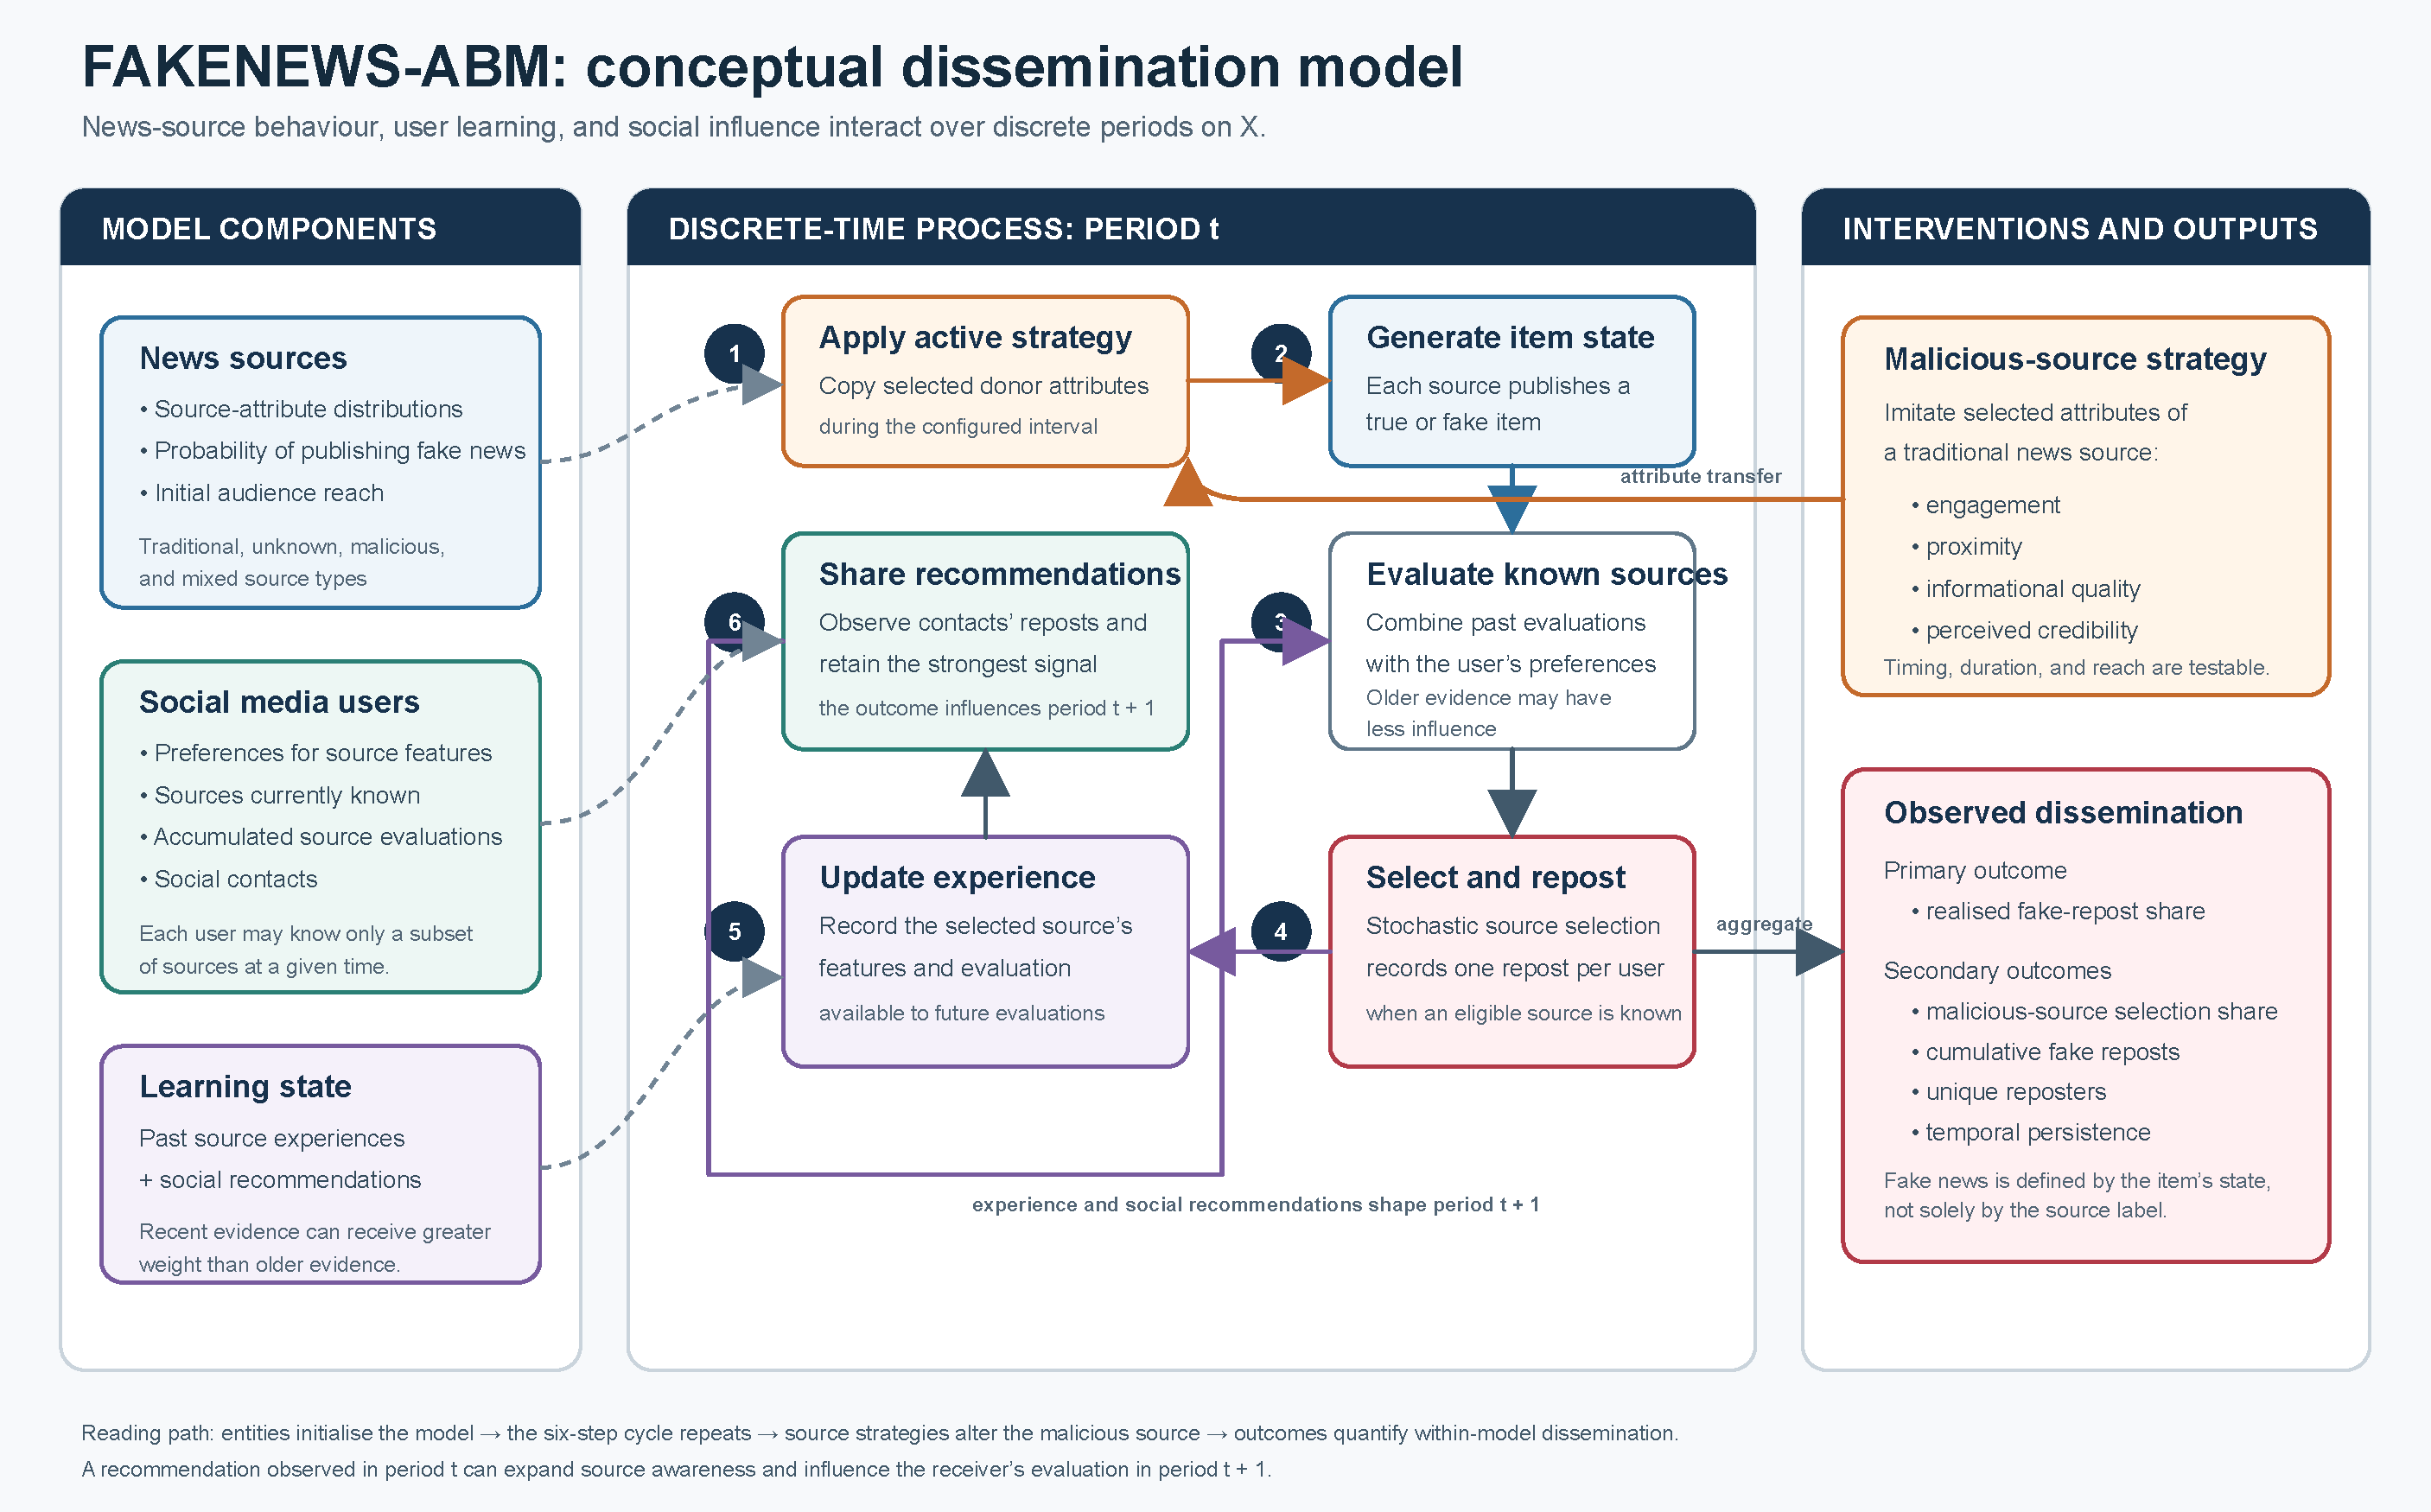
\includegraphics[width=.96\linewidth]{abm-conceptual-model.pdf}
\caption{Conceptual structure of the agent-based model and the feedback from source selection, publication state, and social recommendation.}\label{fig:conceptual}
\end{figure}

Users carry weights indicating the importance assigned to each perceived attribute and to social recommendation. They also retain endorsement events for known sources and have a random set of contacts. Source reach determines whether a source is initially known. With unrestricted reach, all four sources are available; reach-policy experiments vary the malicious source's direct visibility.

\subsection{Process overview and scheduling}

At reset, the simulator constructs users, assigns contacts and visible sources, and generates initial endorsement evidence. During each period: (1) any scheduled source strategy starts or ends; (2) every user aggregates remembered endorsements for known sources; (3) the user probabilistically selects and reposts one source; (4) the selected source independently realizes a true or false publication according to its fixed probability; (5) aggregate and unique-reposter statistics are recorded; and (6) users receive the strongest source recommendation observed among their contacts for use in the following period.

Endorsement contributions are signed and transformed by an exponential base before aggregation. In the principal design, the hard memory window is disabled and each endorsement of age $a$ receives weight
\begin{equation}
w(a)=2^{-a/h},
\end{equation}
where $h=0.33$ periods is the half-life. Truth-sensitive social recommendation penalises a recommendation attached to a false publication and rewards one attached to a true publication. The receiver magnitude is the user's social-recommendation weight multiplied by 0.5. RQ4 replaces these settings with a 25-period hard window or half-lives of 0.33, 1, and 5 periods.

\subsection{Design concepts}

\textit{Heterogeneity} arises from stochastic source attributes, individual evaluation histories, source visibility, and contact networks. \textit{Interaction} occurs through contact-based recommendations. \textit{Adaptation} is represented by probabilistic source choice based on accumulated evidence; malicious sources adapt exogenously through scheduled strategies. \textit{Learning} is path dependent because choices and recommendations add endorsement events. \textit{Stochasticity} enters source visibility, attribute realizations, publication veracity, network construction and source selection. \textit{Observation} records source selections, false-publication states and unique reposters at every period.

Emergence is assessed at the population level: source shares and false-repost exposure are not assigned targets but arise from user-level decisions. Prediction is conditional rather than point forecasting. Sensing is restricted to known sources, personal histories, and contact recommendations. No agent has global network information.

\subsection{Details: initialisation and input parameterisation}

The workbook parameters are informed by aggregated responses from a Chilean survey of 500 X users. The source distributions and mean user weights translate survey constructs into model inputs; source reach values are 81.2\%, 46.7\%, 14.7\%, and 17.5\% for the four source types. We describe this as survey-informed parameterisation, not predictive calibration: the repository does not contain respondent-level microdata or an observed X cascade target against which output parameters were fitted. Consequently, the model supports comparative scenario reasoning but not claims of national representativeness or individual prediction. Survey instrument, sampling dates, recruitment, transformation rules, and ethics information remain author-verification items before submission.

Named strategies group attributes as follows. Engagement copies positive and negative emotion, simple language, sensationalism, entertainment, audiovisual content, and hashtags. Proximity copies political, geographic, and social proximity. Informational camouflage copies information quality and links. Credibility camouflage copies source credibility. The combined strategy copies all four groups from traditional media to the malicious source. Campaign intervals are inclusive; temporary changes are reverted after their final period.

\subsection{Experimental design and statistical analysis}

Table~\ref{tab:design} summarises the study. Every treatment and its control use common seeds. RQ1 compares five permanent strategies with no strategy. RQ2 crosses credibility and informational camouflage with starts at periods 1, 101, and 201 and durations of 25, 100, or the remainder of the run. RQ3 crosses no strategy, credibility, and informational camouflage with reach levels 14.7\%, 10\%, 5\%, 1\%, and 0\%, both with and without social recommendations. RQ4 crosses three contact counts with four memory settings and compares permanent credibility camouflage with control.

\begin{table}[ht]
\centering
\caption{Experimental design.}\label{tab:design}
\begin{tabular}{lrrp{7.4cm}}
\toprule RQ & Conditions & Seeds & Factors \\
\midrule
RQ1 & 6 & 30 & Five source strategies and control \\
RQ2 & 19 & 30 & Strategy, start period, and duration \\
RQ3 & 30 & 30 & Strategy, malicious-source reach, and social recommendation \\
RQ4 & 24 & 15 & Credibility strategy, contacts, and memory \\
\midrule Total & 79 & & 2,010 independent run files \\
\bottomrule
\end{tabular}
\end{table}

For each seed, treatment minus matched control defines the effect. We report means, Student-$t$ 95\% confidence intervals, paired standardised effects ($d_z$), and Holm-adjusted $p$ values within each RQ and outcome family. Effect sizes on shares are expressed in percentage points (pp). Because this is a stochastic simulation experiment, intervals quantify Monte Carlo variability under the encoded model; they do not estimate sampling error for the population of X users.

\subsection{Software execution and reproducibility}

The Java reference implementation, study specification, processed run-level metrics and analysis scripts are open source. The study was run with six concurrent Java processes on a MacBook Pro with an Apple M2 Max processor (12 CPU cores: eight performance and four efficiency), 32 GB RAM, macOS 26.6.1, and OpenJDK 25.0.1. Timestamped study artefacts show an elapsed execution time of approximately 10 h 29 min, from 16 August 2026 at 13:48 to 17 August 2026 at 00:17 (America/Santiago). The public processed dataset reproduces all reported statistics, tables, and figures without the generated workbooks; the code, condition definitions and seeds permit a complete rerun. These materials are available from \ifdefined\ANONYMOUS a public reproducibility repository whose identifying address is omitted here to preserve double-anonymous review\else\url{https://github.com/pleger/FAKENEWS-ABM-News-Source-Strategies}\fi.

\section{Scenario analysis}

\subsection{RQ1: source-imitation strategies}

Figure~\ref{fig:rq1} shows that increasing the malicious source's audience did not automatically increase overall false-news exposure. Informational and credibility camouflage increased malicious-source share by 0.087 pp (95\% CI 0.065--0.109) and 0.048 pp (0.020--0.076), respectively. Combining all attribute groups produced the largest audience effect, 0.471 pp (0.399--0.543), and 17.17 additional unique malicious-source reposters at period 400 (13.74--20.59).

The corresponding average false-repost-share effects were small. The combined strategy added 0.157 pp, but its interval included zero ($-0.017$ to 0.331 pp; Holm $p=0.301$). Proximity alone reduced false-repost share by 0.033 pp ($-0.055$ to $-0.012$; Holm $p=0.017$). In the last 100 periods, however, the combined strategy increased false-repost share by 0.199 pp (0.121--0.277). Thus RQ1 supports audience capture through imitation, particularly combined imitation, but does not support a general one-to-one conversion from source reach to total false-news exposure.

\begin{figure}[ht]\centering

\includegraphics[width=.86\linewidth]{rq1-strategy-effects.png}
\caption{Paired effects of permanent source strategies on average fake-news repost share. Error bars are 95\% $t$ intervals across 30 common seeds.}\label{fig:rq1}
\end{figure}

\subsection{RQ2: timing, duration, and persistence}

Timing and duration mainly changed malicious-source participation. Early permanent informational camouflage produced the largest average source-share gain, 0.087 pp (0.065--0.109), followed by the same strategy beginning at period 101 (0.051 pp) and period 201 (0.038 pp). The pattern is consistent with mechanical exposure time: earlier and longer campaigns provide more periods in which changed attributes can affect choices. A 100-period informational campaign beginning at period 1 added 0.035 pp to average source share, whereas a 25-period campaign added 0.015 pp.

These differences did not translate into robust average false-repost-share effects. Across the 18 treatment cells, all Holm-adjusted intervals for the full-run false-repost outcome included zero. Final-100-period effects were also small, and temporary strategies showed little persistence after removal. The evidence therefore answers RQ2 asymmetrically: timing and duration govern audience opportunity, but under rapid memory decay and truth-sensitive recommendations they do not reliably govern system-wide false-news share.

\begin{figure}[ht]\centering
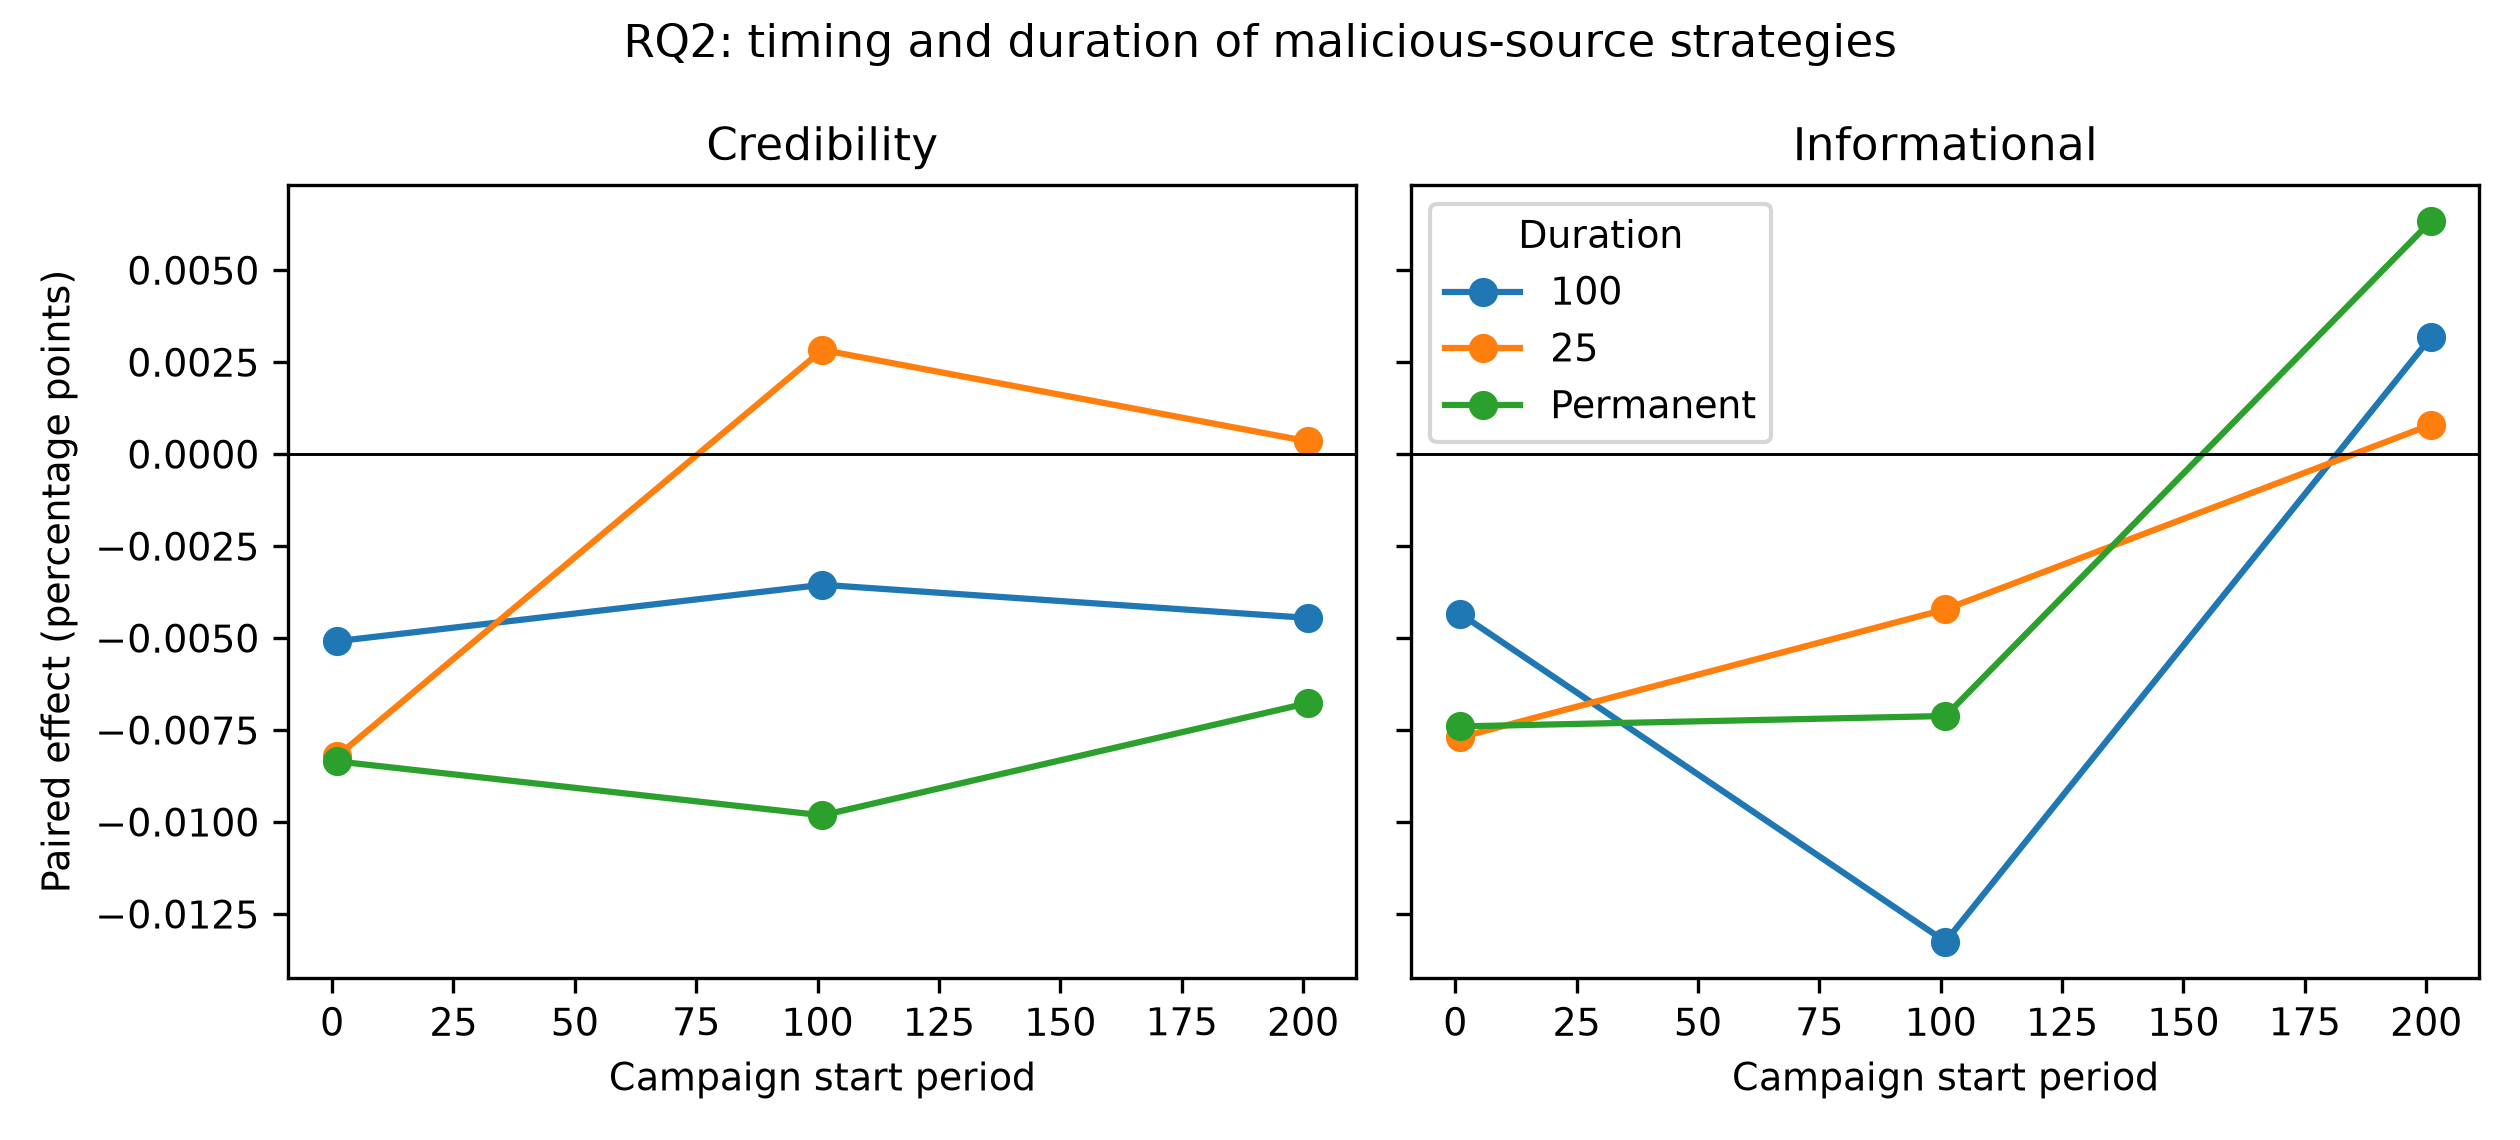
\includegraphics[width=.92\linewidth]{rq2-timing-duration.png}
\caption{Average false-repost-share effects by strategy start and duration. Values are paired against the no-strategy control.}\label{fig:rq2}
\end{figure}

\subsection{RQ3: reach restrictions and social recommendations}

Direct reach restrictions reduced both the malicious source's participation and the incremental effect of camouflage. With social recommendations disabled, informational camouflage added 0.510 pp to false-repost share at 14.7\% reach, 0.355 pp at 10\%, 0.192 pp at 5\%, and 0.047 pp at 1\%; at zero reach its effect was exactly zero. Credibility camouflage followed the same monotonic pattern with smaller effects.

Truth-sensitive social recommendations changed the scale of these effects. At 14.7\% reach, the informational effect fell from 0.510 pp without recommendations to 0.019 pp with recommendations; the credibility effect fell from 0.313 to 0.010 pp. The recommendation mechanism can reveal previously unknown sources, but it also penalises recommendations associated with false publications. In this model the truth-sensitive component dominates, so social interaction does not simply bypass a reach restriction.

The absolute level of false reposts also declined when recommendations were active. For example, the no-strategy condition at 14.7\% reach averaged 14.483\% false reposts without recommendations and 9.820\% with them. Because the recommendation rule explicitly uses publication truth state, this comparison should be interpreted as a modelled policy mechanism rather than evidence about the current algorithm of X.

\begin{figure}[ht]\centering
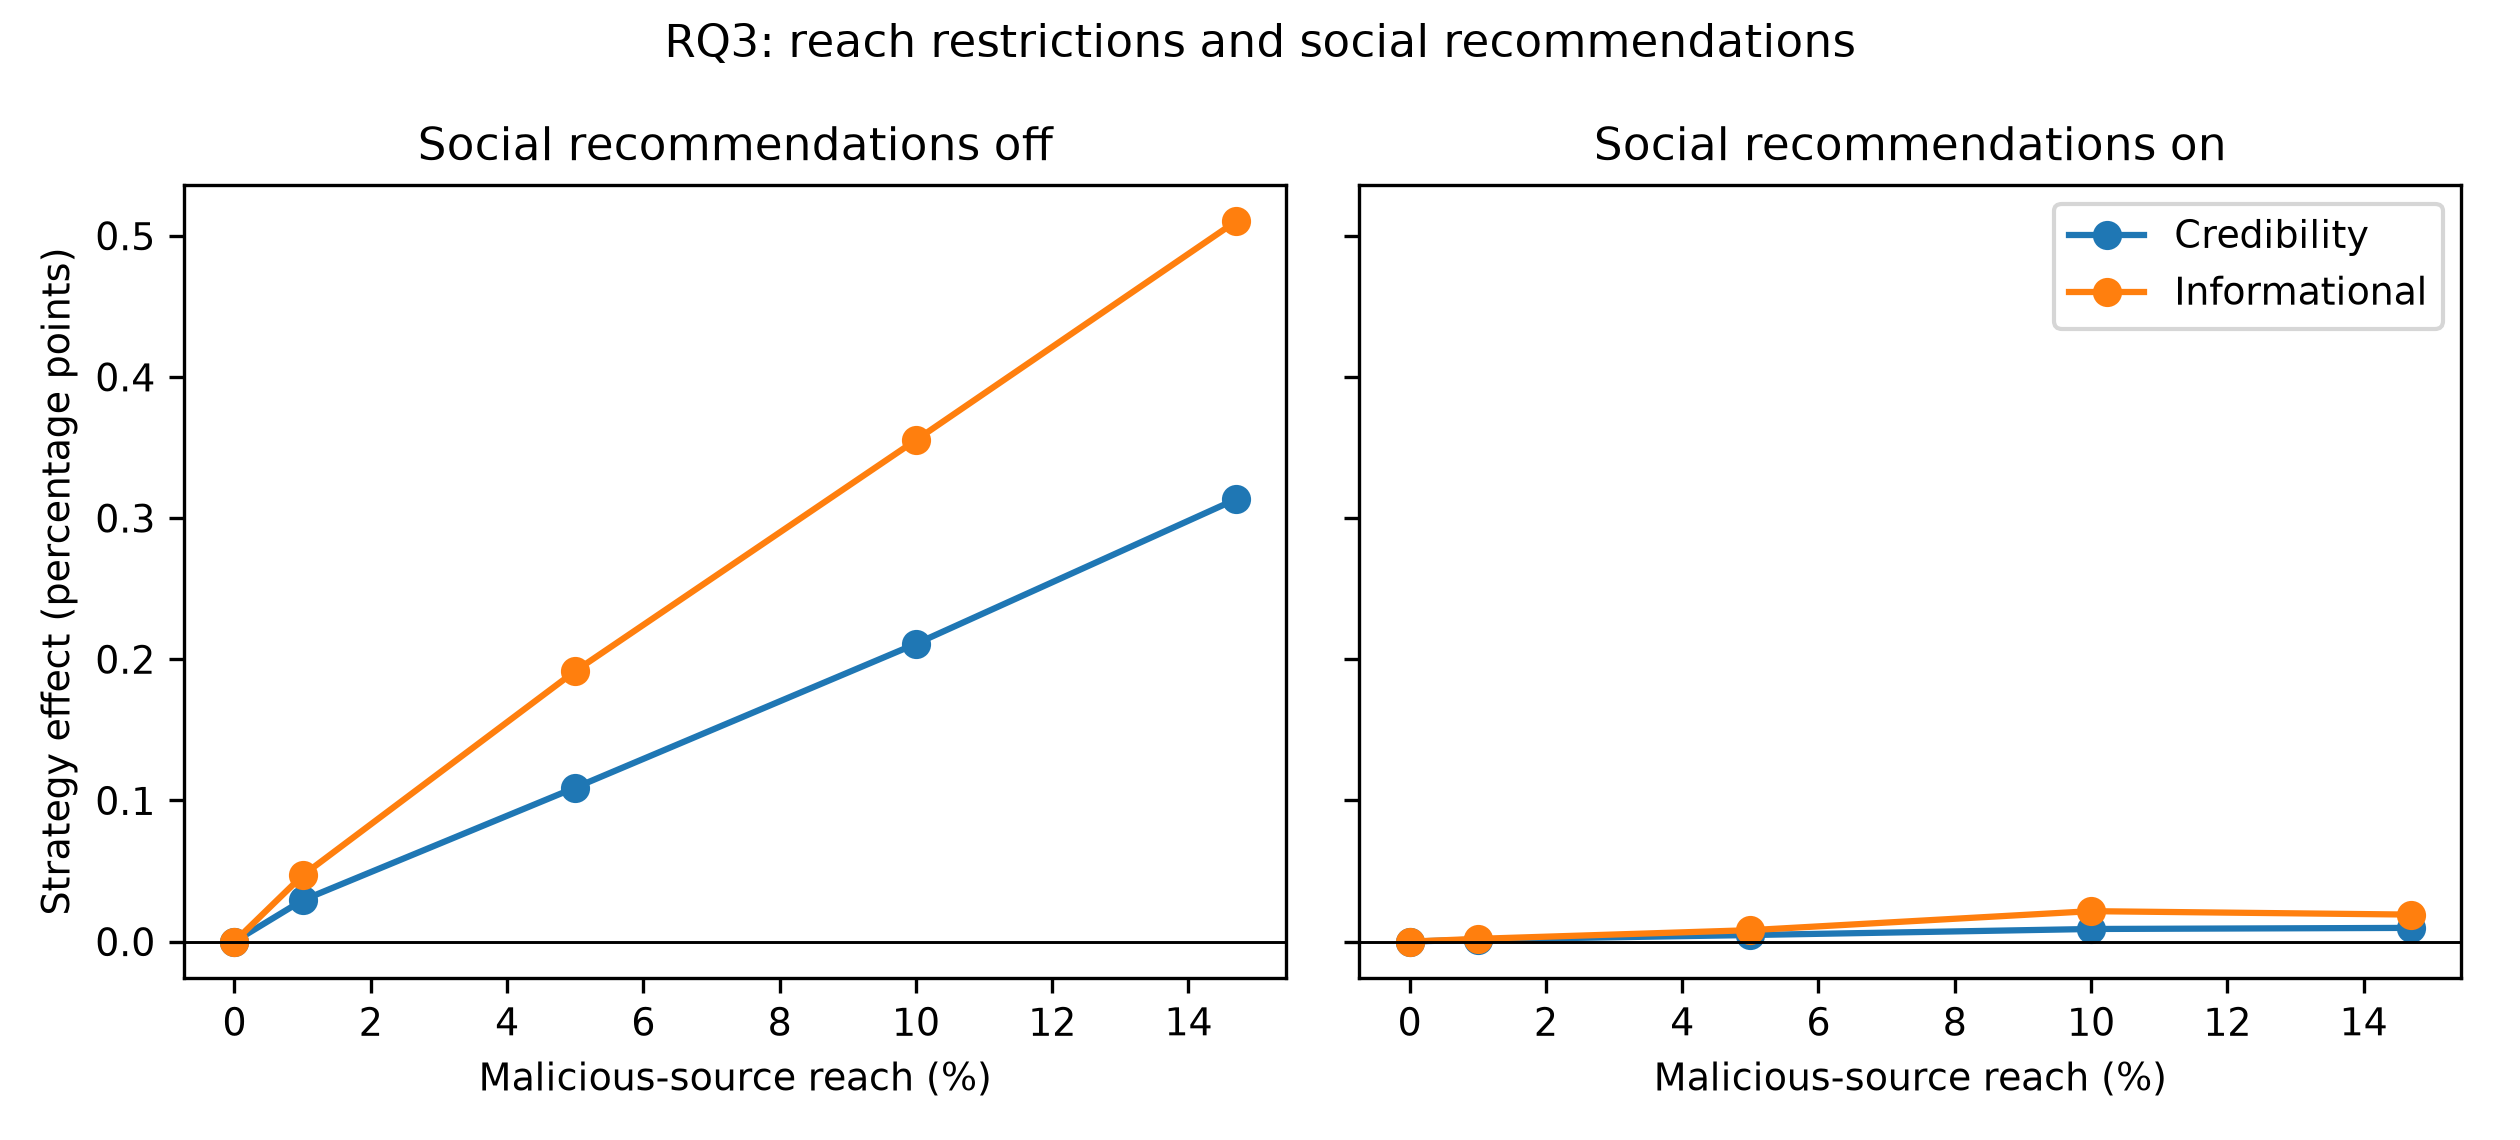
\includegraphics[width=.92\linewidth]{rq3-reach-mitigation.png}
\caption{Strategy effects across malicious-source reach limits, separated by the social-recommendation rule.}\label{fig:rq3}
\end{figure}

\subsection{RQ4: sensitivity and robustness}

Credibility camouflage increased malicious-source share across all twelve memory-connectivity combinations. Effects ranged from 0.043 to 0.295 pp, although the interval for 10 contacts and half-life 0.33 included zero. This supports a qualitatively robust audience-capture conclusion.

The false-repost conclusion was more sensitive. Under a 25-period hard window, credibility camouflage added 0.127--0.145 pp to average false-repost share. With a five-period half-life, effects remained positive at 0.073--0.104 pp. They became smaller with a one-period half-life and indistinguishable from zero under the 0.33-period half-life. Contact count changed magnitude less consistently than memory persistence. RQ4 therefore rejects an unconditional robustness claim for misinformation exposure: whether source camouflage accumulates into additional false reposts depends strongly on how long user evaluations remain influential.

\begin{figure}[ht]\centering
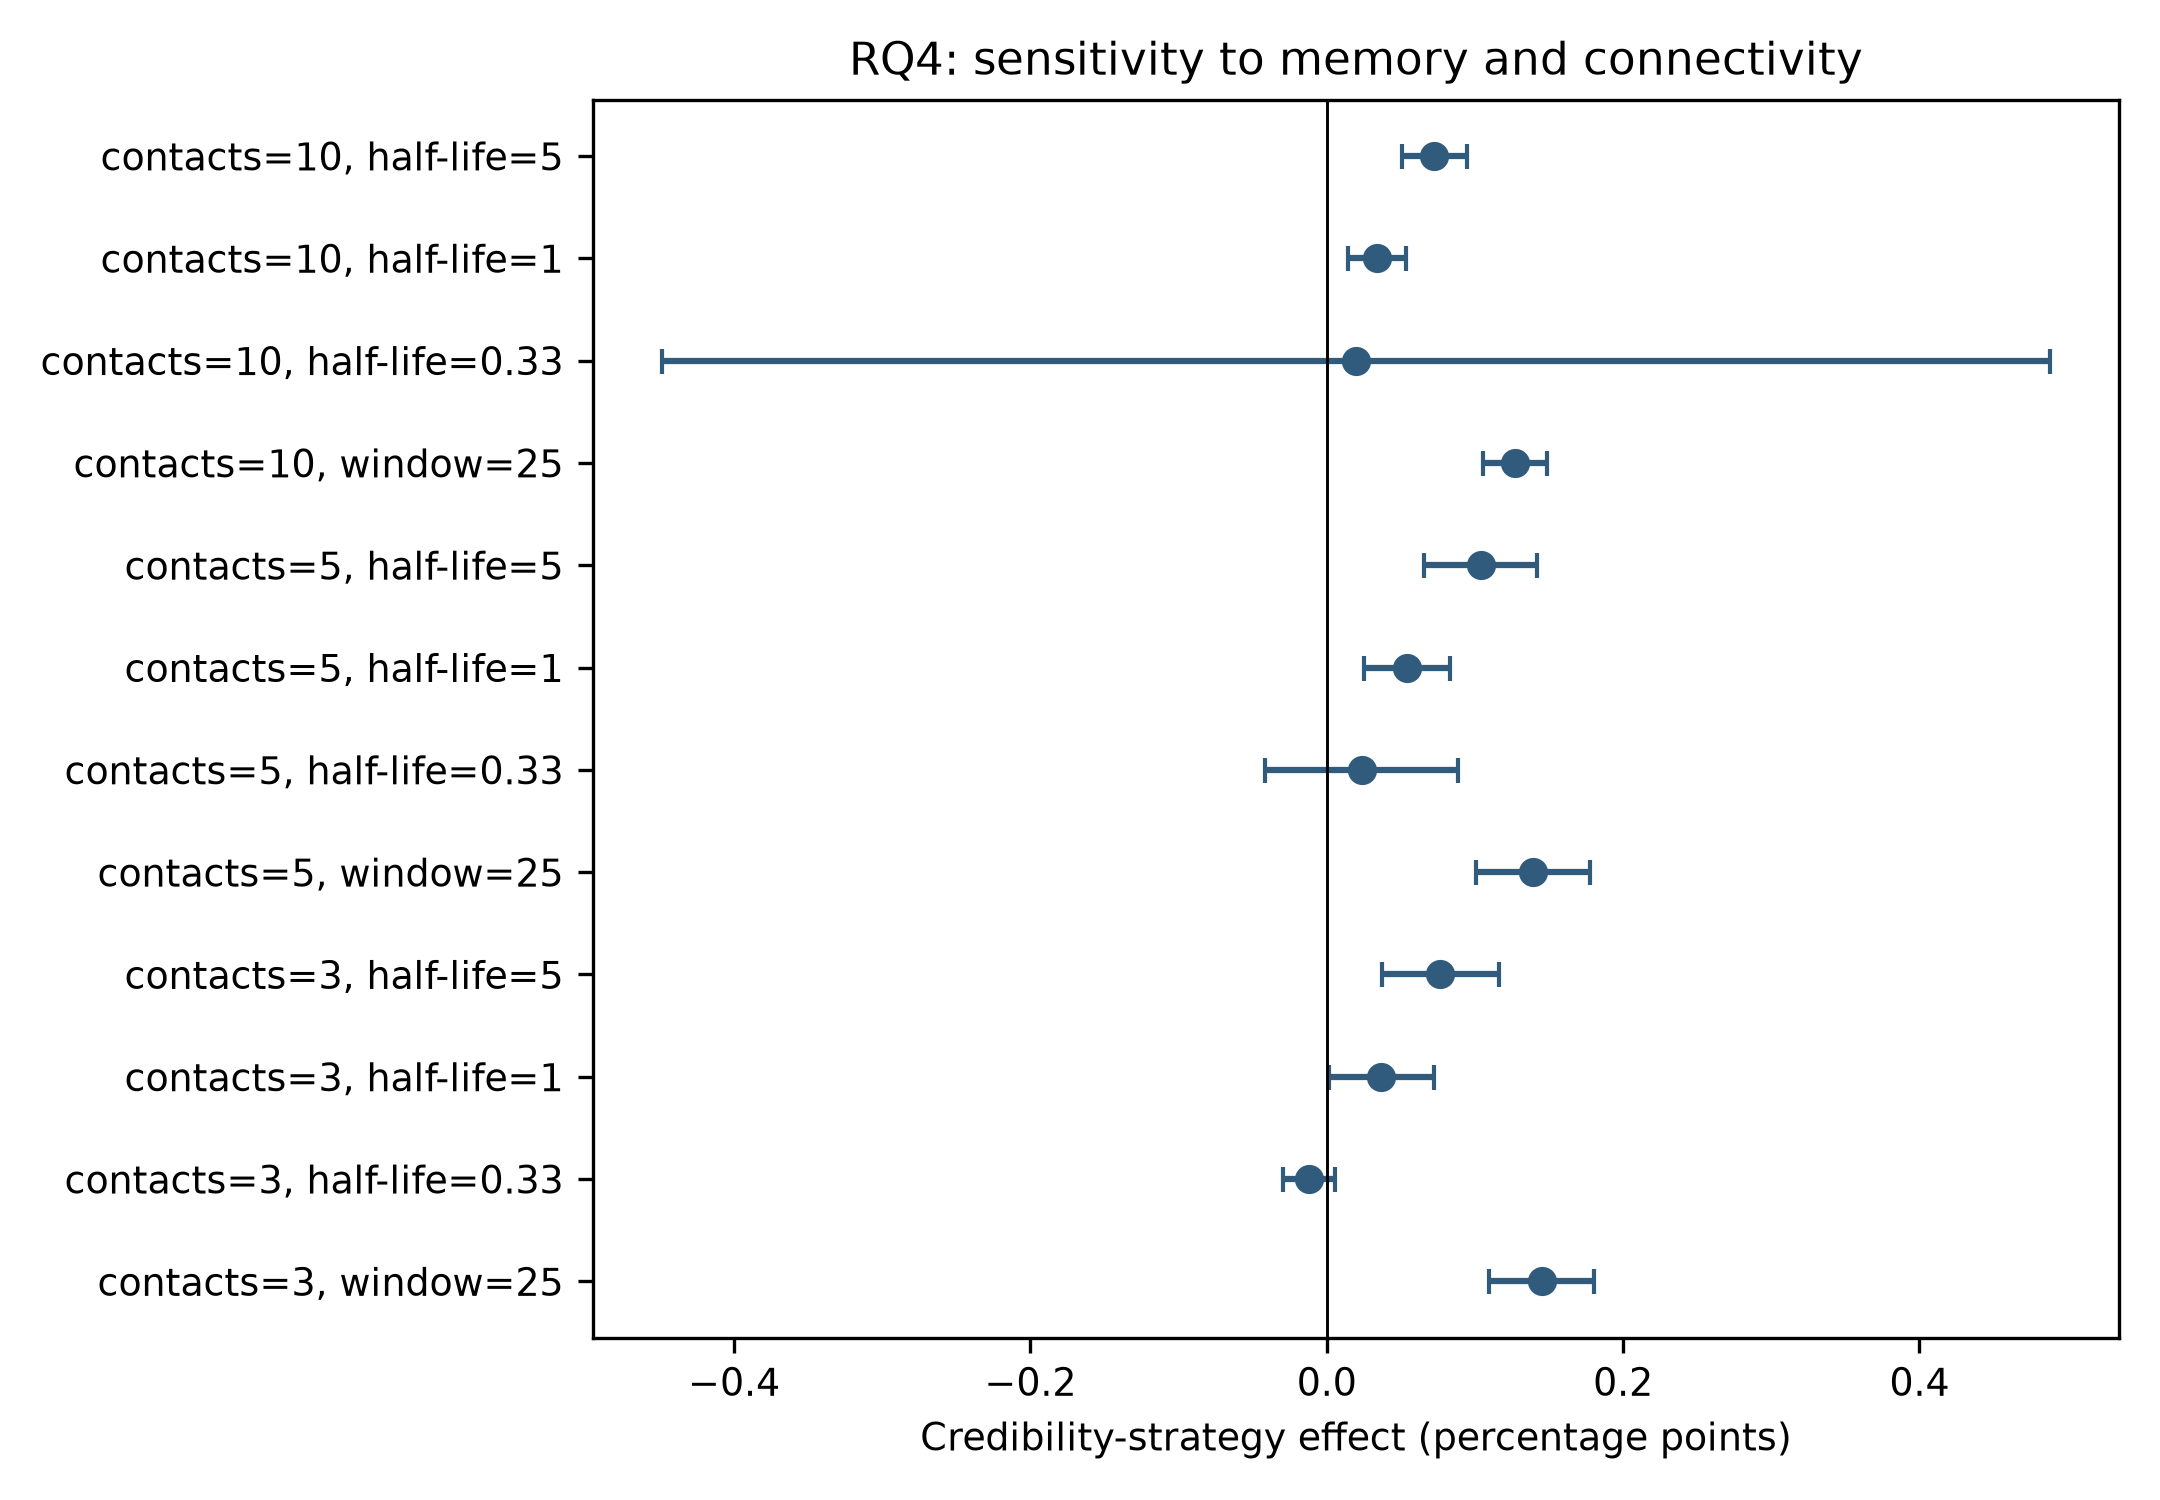
\includegraphics[width=.88\linewidth]{rq4-sensitivity.png}
\caption{Sensitivity of the credibility-camouflage effect on average fake-news repost share to contact count and memory.}\label{fig:rq4}
\end{figure}

\section{Verification and validation}

\subsection{Software verification}

The software separates input loading, agent behaviour, source behaviour, scenario transformation, experiment orchestration, and reporting into components with explicit interfaces. Configuration errors are fatal, including invalid memory combinations, probabilities outside $[0,1]$, unknown strategies, incompatible campaign periods, and missing source attributes. Legacy workbooks remain executable when the new strategy sheet is absent, while the new schema separates perceived credibility from objective fake-news probability.

Automated tests cover configuration defaults and failures, memory decay, truth-sensitive recommendation, strategy resolution, temporary scenario restoration, seeded reproducibility, study planning, and backward compatibility. The final-study analyser adds independent checks at the output boundary. It verified exactly 2,010 unique completed workbooks, 400 ordered periods per analytical sheet, binary publication states, valid population totals, unique condition-seed combinations, and the expected number of conditions per RQ. The analysis itself has unit tests confirming seed-based pairing and confidence-interval calculation.

\subsection{Conceptual and behavioural validation}

The conceptual structure was reviewed against the intended causal narrative: users compare sources, past and social evaluations influence later selection, sources generate publications independently of perceived credibility, and strategies change presentation rather than truthfulness. ODD documentation exposes these assumptions for inspection. The separation of source selection and fake-publication state is also validated in the outputs: strategies can increase source share without proportionally increasing false-repost share.

Input validation is survey-informed. Aggregated responses from 500 Chilean X users provide user weights and source-attribute distributions. Range, probability-sum, source-coverage and schema checks are enforced when the workbook loads. This gives the model an empirical anchor, but it is not external predictive validation because respondent-level data and observed X cascade outcomes were not used to fit and test the simulated diffusion curves.

Behavioural checks include boundary and directional cases. Zero malicious-source reach produces zero direct malicious-source selections and zero strategy effect. Longer memory allows source changes to accumulate more strongly. Truth-sensitive recommendations reduce false-repost exposure relative to recommendation-disabled conditions. RQ4 deliberately varies uncertain memory and connectivity parameters and therefore functions as sensitivity analysis rather than policy evaluation.

The overall validation judgement is \textit{fit for comparative scenario analysis with caveats}. The model can compare mechanisms consistently under controlled conditions. It should not be used to predict the number of false reposts on X, infer causal effects in the platform, or generalise the Chilean survey parameters to other populations without further external validation.

\begin{figure}[ht]\centering
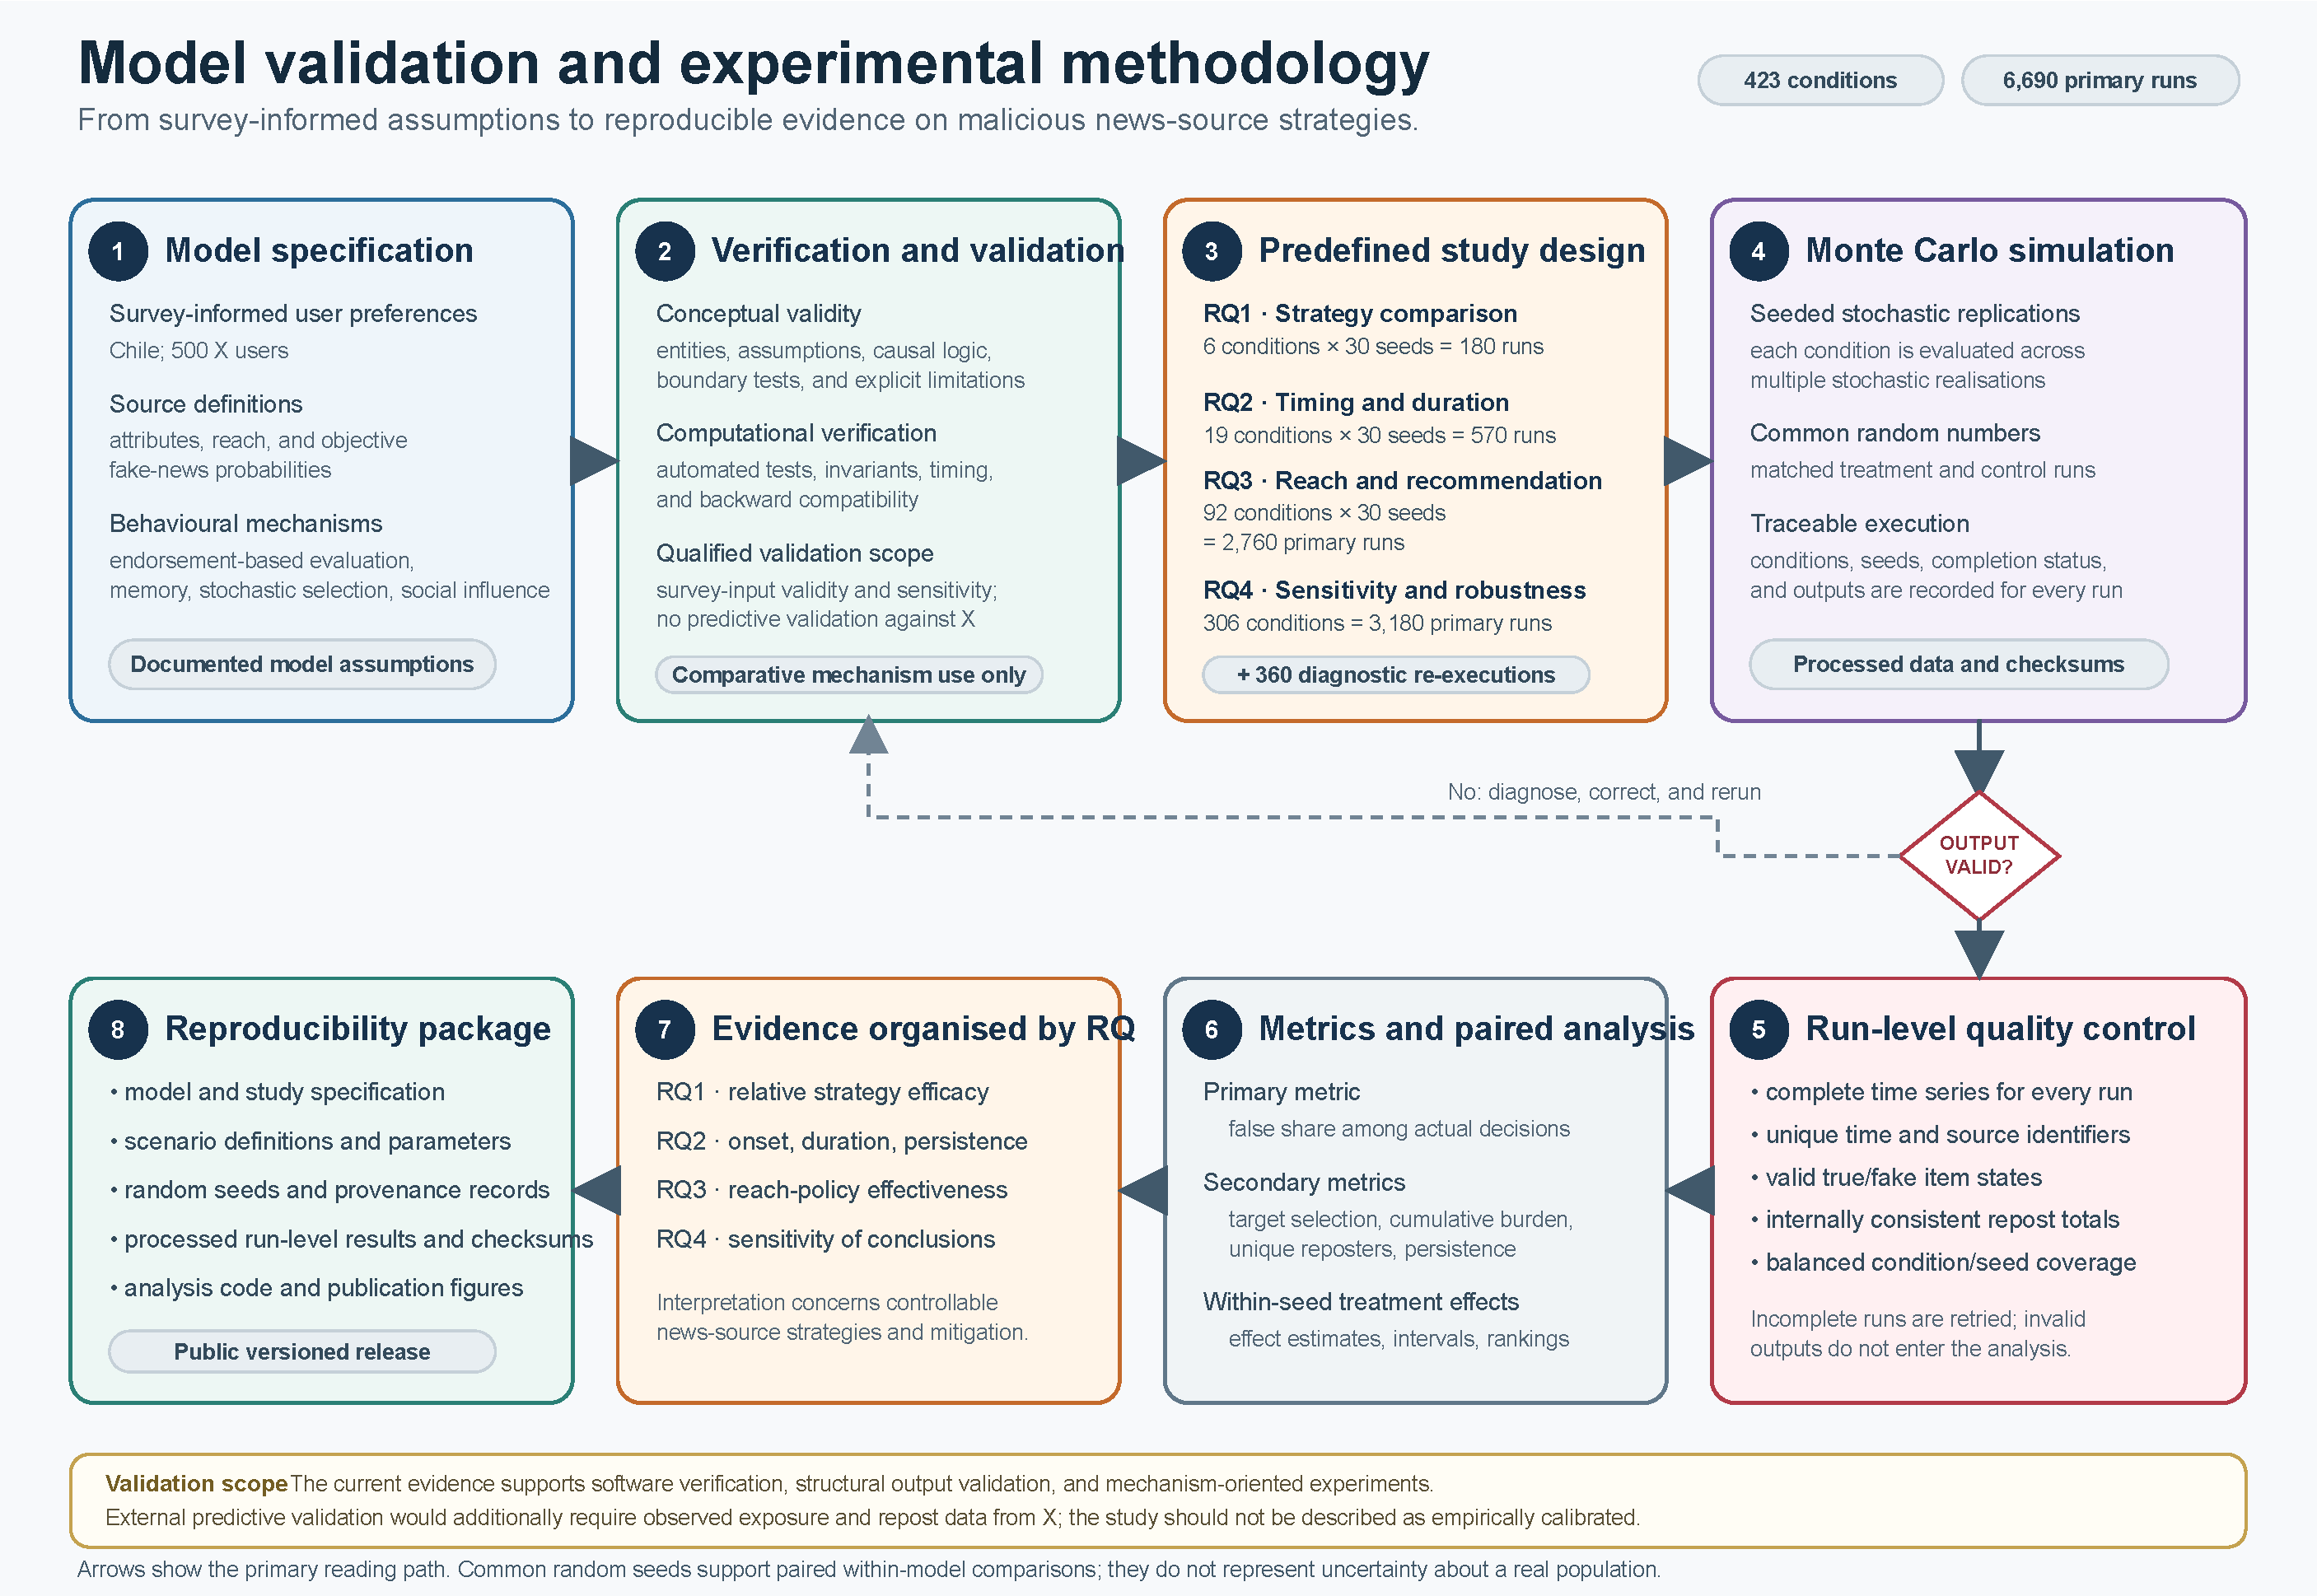
\includegraphics[width=.96\linewidth]{study-validation-methodology.pdf}
\caption{Methodological chain connecting conceptual specification, survey-informed inputs, software verification, scenario experiments, sensitivity analysis, and qualified inference.}\label{fig:validation}
\end{figure}

\section{Discussion and implications}

The central finding is that malicious-source success and misinformation exposure are related but distinct outcomes. A source can gain selection share and unique reposters by resembling traditional media, yet the network-wide false-repost share may barely move when users rapidly discount old information and social recommendations react negatively to false publications. Evaluations of platform policy should therefore report both source-level and content-level indicators. Removing one source metric from a dashboard can conceal displacement or exposure effects elsewhere.

Combined imitation produced the clearest audience gain and a delayed increase in false reposts. This suggests that policies based on a single surface characteristic are vulnerable to multidimensional camouflage. Source assessment should combine provenance, behavioural history, publication-level accuracy and coordination signals instead of relying on appearance alone. The result is compatible with evidence that source-quality judgments can support interventions \citep{pennycook2019}, while extending the question to adaptive source presentation.

Reach governance was the strongest directly controllable mechanism in the experiments. Lower direct visibility monotonically reduced the incremental effect of a malicious strategy, and zero reach eliminated it. This does not imply that account removal is always socially desirable or operationally feasible. Real sources can create new accounts, migrate across platforms, or exploit indirect sharing. The result instead establishes a controlled benchmark: when a platform can reduce initial recommendation and discovery exposure, malicious-source strategy has less opportunity to operate.

Social recommendation requires careful interpretation. Generic word of mouth could amplify harmful information, but the implemented mechanism is truth sensitive: false recommendations generate negative evidence and true recommendations positive evidence. Its protective effect is therefore a design result, not a description of X. A practical implication is that recommendation systems need reliable and timely integrity signals if they are expected to dampen misinformation. Delayed or noisy truth classification could yield different dynamics and should be examined in future scenarios.

Memory sensitivity places a boundary around policy claims. Long-lived evaluations amplify the downstream consequences of camouflage, while rapid decay prevents many effects from accumulating. Memory is not itself a policy variable in the same sense as reach, but interfaces, repeated exposure and ranking can influence how often source signals are refreshed. The sensitivity analysis is valuable precisely because it shows which conclusions survive behavioural uncertainty: audience capture is broadly robust; increased false exposure is not.

Several limitations remain. The network is random and small relative to X, users listen to a fixed number of contacts, and all agents use the same decision architecture. Fake-news probability is source-specific but content is not represented semantically. The Chilean survey supplies aggregate inputs without respondent-level uncertainty, detailed sampling documentation, or an external diffusion target. The platform's proprietary ranking, moderation and bot-detection systems are not reconstructed. Results are therefore mechanism-based counterfactuals rather than forecasts. Future work should incorporate empirical networks, user segments, delayed truth assessment, coordinated sources, account replacement, and calibration/validation against observed cascades while preserving the transparent source-behaviour distinction.

\section{Conclusions}

This section consolidates the answers to the four research questions, identifies the policy conclusions that survive sensitivity analysis, and clarifies the external validation required before predictive use.

This study used an open, survey-informed ABM to evaluate how malicious news sources can imitate trusted-source attributes and how platform-controllable reach and recommendation policies interact with those strategies. Across 6,690 seeded runs in 423 conditions, source camouflage consistently improved audience-related outcomes, with combined imitation producing the largest gain. Campaign timing and duration determined how long the changed source could compete for attention. Immediate perfect truth signals strongly attenuated strategy effects, whereas incomplete, inaccurate or delayed recommendation evidence allowed substantially larger effects. Reach therefore cannot be interpreted independently of the recommendation mechanism that may reveal the source.

The sensitivity experiments provide the qualification needed for policy interpretation. Audience capture remained positive across all structural contrasts. False-exposure effects were less general: memory was the largest influence on combined imitation, several inputs interacted, and credibility camouflage alone seldom produced precise structural exposure effects. Consequently, policy evaluation should not equate malicious-source popularity with misinformation exposure, should use both source- and publication-level measures, and should test recommendation quality and reach governance jointly.

The model is a transparent computational laboratory, not a digital twin of X. Its numerical results are comparative outcomes under the stated model assumptions, not forecasts of X. Its value lies in controlled comparison, explicit assumptions and reproducible uncertainty analysis. External validation with observed X data is the next step required before predictive or population-level claims can be made.

\section*{Acknowledgements}
This work was developed in the context of the PLURALISMO project PLU230018, \textit{Evaluación de Estrategias para Diseminar Fake News Usando Inteligencia Artificial}. The formal acknowledgement wording must be confirmed by all authors before submission.

\section*{Disclosure statement}
The authors report no competing interests. This statement is to be confirmed by all authors.

\section*{Funding}
Project identifier PLU230018 supported this work. The formal funder name and award wording are to be verified before submission.

\section*{Data and code availability}
\ifdefined\ANONYMOUS Code, configuration, analysis scripts and checksummed processed results are available in a public reproducibility repository; its identifying address is withheld here to preserve double-anonymous review.\else The open-source software, study configuration, seeds, run-level processed data and derived analysis artefacts are available at \url{https://github.com/pleger/FAKENEWS-ABM-News-Source-Strategies}. The generated raw workbooks are not tracked, but can be reproduced from the published code, input workbook, condition definitions and seeds.\fi

\section*{Author contributions}
CRediT roles and their allocation are to be confirmed by all authors. Candidate roles are conceptualisation, methodology, software, validation, formal analysis, investigation, data curation, writing---original draft, writing---review and editing, visualisation, supervision, project administration, and funding acquisition.

\section*{Ethics statement}
The simulation uses synthetic agents and aggregate survey-informed parameters. The survey's approval, consent, recruitment and anonymisation statements are to be supplied and verified before submission.

\section*{Generative AI statement}
Generative AI tools were used to assist with analysis-code drafting, language editing, manuscript structuring and document formatting. All model definitions, statistical choices, results, citations and interpretations were reviewed by the authors, who retain full responsibility for the work.

\bibliographystyle{plainnat}
\bibliography{reference}
\end{document}
